
\chapter{Virtual Reference Feedback Tuning - A User Guide}
\label{chap:vrft}

\newcommand{\thetavec}{\underline{\theta}}
\newcommand{\thetaveco}{\underline{\theta_o}}
\newcommand{\thetaveci}{\underline{\theta_i}}

The aim of this chapter is to provide an explanation of the Virtual Feedback Reference Tuning method (henceforth referred to as VRFT). This method allows for the direct identification of a transfer function of the controller, using a single set of data and without requiring specific experiments or iterations. 

\section{Introduction}
\label{sec:vrft_introduction}

It is often the case when developing a control system for a system that no accurate mathematical description of the plant is available. Thus, before any work can be undertaken it is necessary to identify a model of the plant. Alternatively, simple heuristic methods can be applied to derive a workable controller. This is the case for example of the Ziegler and Nichols procedure. However, these approaches are rigid and do not allow the designer to easily tune the resulting controllers. 

VRFT, without requiring any identification of the plant, allows the designer to easily tune a controller to fit any achievable performance criterion.

\section{A Birds Eye View}
\label{sec:vrft_birds_eye_view}

In VRFT the aim is identify the parameters of a controller such that the complementary sensitivity of the system aligns with a \emph{reference model}. This model describes the desired behaviour of the closed loop system. 

\begin{figure}[!ht]
    \documentclass[convert={outext=.png}]{standalone}
\usepackage{tikz}

% Compile with: lulatex -shell-escape vrft_block_diagram_standalone.tex

\tikzset{
	block/.style  = {draw, fill=white, rectangle, minimum height=3em, minimum width=5em, node distance = 2cm},
	sum/.style    = {draw, fill=white, circle, node distance=1cm},
	input/.style  = {coordinate},
	output/.style = {coordinate},
	hidden/.style  = {coordinate},
}

\begin{document}
	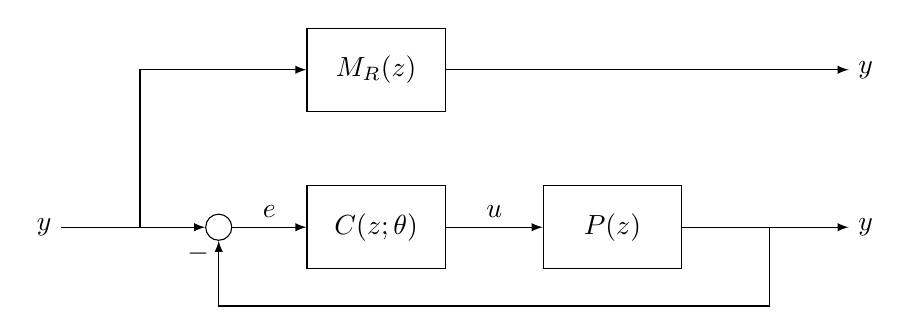
\begin{tikzpicture}[auto, >=latex]
		% Draw the main control loop nodes
		\draw
		node[input] (input) {}
		node[hidden, right of = input     ] (inputfork) {}
		node[sum   , right of = inputfork ] (sum) {}
		node[block , right of = sum       ] (controller) {$C(z; \theta)$}
		node[block , right of = controller, node distance = 3cm] (plant) {$P(z)$}
		node[hidden, right of = plant     , node distance = 2cm] (outputfork) {}
		node[output, right of = outputfork] (output) {}
		node[hidden, below of = plant     ] (retroaction) {};
		
		% Draw the reference model nodes
		\draw
		node[block , above of = controller] (refmodel) {$M_R(z)$}
		node[coordinate, right of = refmodel, node distance = 6cm] (refoutput) {};
		
		% Connect everything together
		\draw[->] node[left] {$y°$} (input) -- (inputfork)  -- (sum);
		\draw[->] (sum) -- (controller) node[midway] {$e$};
		\draw[->] (controller) -- (plant) node[midway] {$u$};
		\draw[->] (plant) -- (outputfork) -- (output) node[right] {$y$};
		
		\draw[->] (outputfork) |- (retroaction) -| node[pos=0.9] {$-$} (sum);
		
		\draw[->] (inputfork) |- (refmodel);
		\draw[->]  (refmodel) -- (refoutput) node[right] {$y$};
	\end{tikzpicture}
\end{document}

    \caption{Control and reference model}
    \label{fig:vrft_bd}
\end{figure}

The VRFT algorithm calculates the transfer function of the controller \( C(z;\ \thetavec) \) by solving a parameter identification problem. If both the input and the output of the controller are known then it is possible to find an optimal parameter vector, \( \hat{\thetavec} \), that minimises the distance between the reference model and the closed loop transfer function of the system. The input and the output of the controller are respectively, the tracking error \( e(t) \) and the plant input \( u(t) \).

Assume that we have on hand a set of \( u \) and \( y \) measurements on the plant. If the controller achieves the optimisation goal and the closed loop transfer function of the system is equal to the reference model then, both systems, when fed the same input, will produce the same output. 

Let \( M_R(z) \) be the reference model. If the reference signal, \( \bar{r}(t) \) is calculated such that: 

\begin{equation}
    y(t) = M_R(z) \cdot \bar{r}(t)
\end{equation}

then the tracking error is simply:

\begin{equation}
    e(t) = \bar{r}(t) - y(t)
\end{equation}

Since both the input, \( e(t) \), and the output, \( u(t) \), of the controller are known the identification can be performed and the optimal controller can be retrieved.

\section{A Rigorous Explanation}
\label{sec:vrft_rigorous_expl}

We assume that the plant is a linear SISO dynamical system described by a rational transfer function \( P(z) \) that is unknown to the designer. 

We also assume that a set of open-loop input/output data has been collected during an experiment on the plant. The only requirement for this experiment is that it must be aggressive enough to excite the system over the entirety of the frequency range of interest. The experiment provides us 2 vectors of data-points.

\begin{align*}
    \underline{u} &= \left\{ u_0,\ u_1,\ u_2,\ \ldots\ , u_n \right\} \\
    \underline{y} &= \left\{ y_1,\ y_2,\ y_3,\ \ldots\ , y_n \right\}
\end{align*}

The designer must also choose a reference model that describes the desired closed-loop behaviour of the system. Great care should be taken here to choose a model that is physically achievable given the physical constraints of the system. If the reference model is unachievable the controllers will be of very limited use. Let this reference model be \( M_R(z) \).

Finally, the designer must choose a class of controllers to tune. The controller class is reduced to the set of controllers that can be expressed as a linear combination of linear, discrete time, transfer functions. This controller class takes the form:

\begin{equation}
    C(z;\ \thetavec) = \beta^T(z) \cdot \thetavec
\end{equation}

\noindent
Where \( \beta^T(z) \), the vector of linear transfer functions is

\begin{equation*}
    \beta^T(z) = \left[ \beta_1(z),\ \beta_2(z)\ \ldots\ \beta_n(z) \right]^T
\end{equation*}

\noindent
and \( \thetavec \), the parameter vector is 

\begin{equation*}
    \thetavec = \left[ \theta_1,\ \theta_2\ \ldots\ \theta_n \right]^T
\end{equation*}

The control objective is the minimisation of the following performance criterion:

\begin{equation}
    \begin{aligned}
        J_{MR}(\thetavec) 
            &= \left \Vert \left( \frac{P(z)C(z;\ \theta)}{1 + P(z)C(z;\ \theta)} - M_R(z) \right) W(z) \right \Vert_2^2 \\
            &= \left \Vert \left( T(z) - M_R(z) \right) W(z) \right \Vert_2^2
    \end{aligned} 
    \label{eq:control_obj_mr}   
\end{equation}

\noindent
Where \( T(z) \) is the complementary sensitivity function of the system. The control objective simply minimises the difference between the closed-loop transfer function and the reference model scaled by an appropriate weighting function. This allows the designer to emphasize or de-emphasize performance in certain frequency bands.

The choice of the weighting function \( W(z) \) is left to the designer. For many cases \( W(z) = 1 \) is sufficient. 

The frequency domain representation of this criterion is

\begin{equation}
    J_{MR}(\thetavec) =  \frac{1}{2\pi} \int_{-\pi}^{\pi} \left| \frac{PC(\thetavec)}{1 + PC(\thetavec)} - M \right|^2 \left| W \right|^2 d\omega
    \label{eq:jmr_freq}
\end{equation}

An optimal choice of the controller would produce a closed loop transfer function \( T(z) = M_R(z) \) such that

\begin{equation}
    y(t) = T(z) \cdot \bar{r}(t) = M_R(z) \cdot \bar{r}(t)
    \label{eq:ref_equals_compl_sens}
\end{equation}

from which we deduce

\begin{equation}
    \bar{r}(t) = \frac{1}{M_R(z)} \cdot y(t)
    \label{eq:reference_signal}
\end{equation}

The signal \( \bar{r}(t) \) is the \emph{virtual reference} signal, the namesake of the method. It was not used to generate the output \( y(t) \) and only exists as a tool used in the identification of the optimal controller. 

We can write the tracking error of the closed loop system as

\begin{equation}
    \begin{aligned}
        e(t) &= \bar{r}(t) - y(t) \\ 
             &= \bar{r}(t) \cdot (1 - M_R(z))
    \end{aligned}
    \label{eq:tracking_error}
\end{equation}

The optimal controller must be such that when fed the reference signal it produces the measured input \( u(t) \), that is to say 

\begin{equation}
    u(t) = C(z;\ \hat{\thetavec}) \cdot \bar{r}(t)
\end{equation}

\noindent
where \( \hat{\thetavec} \) is the optimal parameter vector. However, directly minimising \( J_{MR}(\theta) \) is non trivial. We will instead first concentrate on a different minimisation objective before showing that is asymptotically equivalent to \( J_{MR}(\theta) \).

Apply a filter \( L(z) \) to the data. The choice of the filter will be detailed at a later time.  The two filtered datasets are

\begin{align}
    e_L(t) &= L(z) \cdot e(t) \\
    u_L(t) &= L(z) \cdot u(t)
\end{align}

Consider the following performance criterion: 

\begin{equation}
    J^N_{VR}(\thetavec) = 
        \frac{1}{N} \sum_{t=1}^{N} \left( u_L(t) - C(z;\ \thetavec) \cdot \ e_L(t) \right)^2 
\end{equation}

Through simple transformations it is possible to rewrite it as

\begin{equation}
    \begin{aligned}
        J^N_{VR}(\thetavec)
            &= \frac{1}{N} \sum_{t=1}^{N}\left( u_L(t) - \beta^T(z)\thetavec \cdot e_L(t) \right)^2 \\
            &= \frac{1}{N} \sum_{t=1}^{N}\left( u_L(t) - \varphi_L^T(t)\thetavec \right)^2, \quad \varphi_L = \beta^T(z) \cdot  e_L(t)
    \end{aligned}    
\end{equation}


Since this criterion is quadratic in \( \thetavec \) the optimal parameter vector \( \hat{\thetavec} \) is an explicit function of the data

\begin{equation}
    \hat{\thetavec}_N 
        = \left[ \sum_t \phi \cdot \phi(t)^T \right]^{-1} \sum_t \phi_t \cdot u(t) 
\end{equation}

If \( u(t) \) and \( y(t) \) can be considered realisations of stationary stochastic processes then as the amount of data grows, \( N \rightarrow \infty \), the minimum \( \hat{\theta}_N \) of \( J^N_{VR}(\thetavec) \) converges to the minimum of \( J_{VR}(\thetavec) \), \( \hat{\thetavec} \).

\begin{equation*}
    \argmin_{\thetavec_N} J^N_{VR}(\thetavec_N) = \argmin_{\thetavec} J_{VR}(\thetavec)
\end{equation*}

This allows us to write that

\begin{equation}
    \begin{aligned}
        J_{VR}(\theta) &= E \left[ \left( u_L(t) - C(z;\ \thetavec)e_L(t) \right)^2 \right] \\
                       &= E \left[ \left( L(z) \cdot \left\{ u(t) - C(z;\ \thetavec)e(t) \right\} \right)^2 \right]
    \end{aligned}
\end{equation}

The dependency on \( e(t) \) can be removed in order to make the criterion depend only on the initial data. As previously noted in equation \ref{eq:reference_signal} the virtual referrence signal is  

\begin{equation}
    \begin{aligned}
        \bar{r}(t) &= \frac{1}{M_R(z)} \cdot y(t) \\
                   &= \frac{1}{M_R(z)} \cdot P(z) \cdot u(t)
    \end{aligned}
    \label{eq:reference_signal_in_u}
\end{equation}

In addition, as shown in equation \ref{eq:tracking_error} the tracking error can be expressed as

\begin{equation*}
    e(t) = \bar{r}(t) \cdot (1 - M_R(z))
\end{equation*}

We can substitute equation \ref{eq:reference_signal_in_u} into the expression of \( e(t) \) which yields 

\begin{equation}
    \begin{aligned}
        e(t) = \frac{1 - M_R(z)}{M_R(z)} \cdot P(z) \cdot u(t)
    \end{aligned}
\end{equation}

By substituting this new expression for \( e(t) \) into \( J_{VR} \) we can rewrite it as

\begin{equation}
    \begin{aligned}
        J^N_{VR}(\theta) 
            &= \frac{1}{N} \sum_{t=1}^{N} \left[ u_L(t) - C(z;\ \thetavec) \cdot \frac{1 - M_R(z)}{M_R(z)} \cdot P(z) \cdot u_L(t) \right]^2 \\
            &= \frac{1}{N} \sum_{t=1}^{N} \left[ L(t) \cdot \left( 1 - C(z;\ \thetavec) \cdot \frac{1 - M_R(z)}{M_R(z)} \cdot P(z) \right) \cdot u(t) \right]^2
    \end{aligned} 
    \label{eq:jvr}
\end{equation}

As shown in equation \ref{eq:ref_equals_compl_sens}, the reference model \( M_R(z) \) is equal to the closed loop transfer function of the system. 

\begin{equation}
    T(z) = M_R(z) = \frac{P(z) C_0(z)}{1 + P(z) C_0(z)} 
    \label{eq:ref_in_pc}
\end{equation}

Where \( C_0(z) = C(z, \hat{\thetavec}) \) is a transfer function that perfectly solves the model matching problem. We also observe that 

\begin{equation}
    \begin{aligned}
        1 - M_R(z) &= \frac{1 + P(z) C_0(z) - P(z) C_0(z) }{1 + P(z) C_0(z)} \\
                 &= \frac{1}{1 + P(z)C_0(z)}
    \end{aligned}
    \label{eq:1_minus_ref_in_pc}
\end{equation}

From which

\begin{equation}
    \begin{aligned}
         1 - C(\theta) \cdot \frac{1 - M_R}{M_R} \cdot P 
            &= \frac{1}{M_R} \left( M_R - P C(\thetavec) \left( 1 - M_R \right) \right) \\
            &= \frac{1}{M_R} \left( \frac{P C_0}{1 + P C_0} - \frac{P C(\thetavec)}{1 + P C_0} \right) \\
            &= \frac{1}{M_R} \left( P \cdot \frac{C_0 - C(\thetavec)}{1 + P C_0} \right) \\
            &= \frac{1}{M_R} \cdot P \cdot \left( C_0 - C(\thetavec) \right) \left( 1 - M_R \right)
    \end{aligned}
\end{equation}

If we substitute the previous result into the expression of the control objective derived in equation \ref{eq:jvr} we can rewrite it in a more convenient form

\begin{equation}
    J^N_{VR}(\thetavec) = E \left[ \left( P \cdot \frac{C_0 - C(\thetavec)}{1 + P C_0} \cdot \frac{L}{M} \right)^2 \right]
\end{equation}

The frequency domain representation of this criterion is

\begin{equation}
    \begin{aligned}
        J_{VR}(\theta) 
            &= \frac{1}{2\pi} \int_{-\pi}^{\pi} \left| P \cdot \frac{C_0 - C(\thetavec)}{1 + P C_0} \cdot \frac{L}{M} \right|^2 \Phi_u \ d\omega \\
            &= \frac{1}{2\pi} \int_{-\pi}^{\pi} \left| \left( \frac{PC_0}{1 + P C_0} - \frac{PC(\thetavec)}{1 + P C_0} \right) \cdot \frac{L}{M} \right|^2 \Phi_u \ d\omega
    \end{aligned}
\end{equation}

\noindent
where \( \Phi_u \) is the power density of the plant input \( u(t) \). If \( C_0(z) \in C(z;\ \thetavec) \) and \( J_{VR}(\thetavec) \) has a unique minimum then minimising \( J_{VR}(\thetavec) \) gives \( C_0(z) \) for any choice of the filter \( L(z) \).

The expression of the initial control objective in frequency domain \( J_{MR}(z) \) as given in equation \ref{eq:jmr_freq} is

\begin{equation}
    \begin{aligned}
        J_{MR}(\thetavec) 
            &=  \frac{1}{2\pi} \int_{-\pi}^{\pi} \left| \frac{PC(\thetavec)}{1 + PC(\thetavec)} - M_R \right|^2 \left| W \right|^2 d\omega \\
            &=  \frac{1}{2\pi} \int_{-\pi}^{\pi} \left| \frac{PC(\thetavec)}{1 + PC(\thetavec)} - \frac{PC_0}{1 + PC_0} \right|^2 \left| W \right|^2 d\omega
    \end{aligned}
\end{equation}

\noindent
Note the similarities between the two criteria. If the filter were to be set to

\begin{equation}
    \left| L \right|^2 = \left| \frac{MW}{1 + PC(\thetavec)} \right|^2 \cdot \frac{1}{\Phi_u},\quad \forall \omega \in \left[ -\pi,\ \pi \right]
\end{equation}

\noindent
Then \( J_{VR}(\thetavec) = J_{MR}(\thetavec) \) and as a consequence \( \hat{\thetavec} \) is a global minima of \( J_{MR}(\thetavec) \) as well as a global minima of \( J_{VR}(\thetavec) \). However this choice of \( L(z) \) is not practical since \( P(z) \) is not known. The method solves this problem by using the following filter

\begin{equation}
    \left| L \right|^2 = \left| \left(1 - M \right) \cdot MW \right|^2 \cdot \frac{1}{\Phi_u},\quad \forall \omega \in \left[ -\pi,\ \pi \right]
\end{equation}

\noindent
All the quantities on the right hand side of this filter are known. The power density \( \Phi_u \) is only known when the input signal has been chosen by the designer however in the general case it can be estimated.

This filter can be rewritten as

\begin{equation}
    \left| L \right|^2 = \left| \frac{MW}{1 + PC_0} \right|^2 \cdot \frac{1}{\Phi_u},\quad \forall \omega \in \left[ -\pi,\ \pi \right]    
\end{equation}

\noindent
Hence, this choice of \( L(z) \) is equivalent to substituting \( \left| 1 + PC(\thetavec) \right|^2 \) with \( \left| 1 + PC_0 \right|^2 \), a sensible choice if, as required, \( C(\thetavec) \) is a good approximation of \( C_0 \).

In summary, by a judicious choice of the pre-filter \( L(z) \) it is possible to change the optimisation problem to make it purely quadratic in \( \thetavec \) which makes the optimisation problem trivial to solve. 

\section{Extension to Cascade Control}
\label{sec:vrft_cascade_control}

The VRFT algorithm can be extended to cascade control system with a little extra work. It can in fact be extended to tune both the inner and the outer controller at the same time using the same dataset.

\begin{figure}[!h]
    \documentclass[convert]{standalone}

\usepackage{graphics}
\usepackage{amsmath}
\usepackage{tikz}

\begin{document}
	\begin{figure}
		\centering
		\input{cascade_vrft.tikz}
		\caption{Cascade VRFT control scheme}
	\end{figure}
\end{document}

    \caption{Control and reference model}
    \label{fig:vrft_cascade_bd}
\end{figure}

We assume that the a set of open loop measurements have been taken during an experiment on the plant. The plant input signal \( u(t) \) must be measured as well as the inner and outer plant outputs \( y_i(t) \) and \( y_o(t) \). The designer should thus have 3 vectors of data-points available

\begin{align*}
    \underline{u} &= \left\{ u_0,\ u_1,\ u_2,\ \ldots\ , u_n \right\} \\
    \underline{y_i} &= \left\{ y_{i_1},\ y_{i_2},\ y_{i_3},\ \ldots\ , y_{i_n} \right\} \\
    \underline{y_o} &= \left\{ y_{o_1},\ y_{o_2},\ y_{o_3},\ \ldots\ , y_{o_n} \right\}
\end{align*}

The designer must also choose two reference models to describe the desired performance of the inner and outer loops. Let \( M_{R_i} \) be the reference models of the inner loop and \( M_{R_o} \) be the reference models of the outer loop.

The control system designer must also chose two families of controllers \( \left\{ C(z;\ \thetaveci) \right\} \) and \( \left\{ C(z;\ \thetaveco) \right\} \) for the inner and outer loops. 

The requirements on the reference models and the controller families are not changed with regards to the standard VRFT method.

The inner controller can be tuned immediately using standard VRFT. The input/output data required for this is available and the only requirement on the inner loop is that it be as close as possible to the reference model. 

The outer loop is slightly more complex. To apply the VRFT method on the outer loop we consider the entire block from \( r_i(t) \) to \( y_o(t) \) as our \emph{plant}. The virtual reference \( r_i(t) \) is unknown however it can be calculated quite simply

\begin{equation}
    r_i(t) = e_i(t) + y_i(t)
\end{equation}

The output \( y_i(t) \) is part of our initial dataset and is known. The inner tracking error is unknown but can be calculated as 

\begin{equation}
     e_i(t) = C(z;\ \thetaveci)^{-1} \cdot u(t)
 \end{equation} 

 Thus, the virtual reference input for the outer loop is

 \begin{equation}
     r_i(t) = C(z;\ \thetaveci)^{-1} \cdot u(t) + y_i(t)
 \end{equation}

 The outer controller can then be easily tuned with the standard VRFT using as input \( r_i(t) \) and as output \( y_o(t) \). 

 The calculation of \( r_i(t) \) is only possible if \( C(z;\ \thetaveci) \) has no unstable zeros. If that is not the case and \( C(z;\ \thetaveci) \) is non-minimum phase then \( C(z;\ \thetaveci)^{-1} \) will be unstable and the inner tracking error \( e_i(t) \) will be meaningless. This is often the case when the requirements on the inner loop are unreachable. 


